%%%% Small single column format
\documentclass[anonymous=false, %
               format=acmsmall, %
               review=true, %
               screen=true, %
               nonacm=true]{acmart} 


\usepackage[ruled]{algorithm2e} 
%\usepackage{parskip}
\usepackage{backnaur}
% \usepackage{jlcode}  
\usepackage{todonotes}
\usepackage{alphabeta}
% \usepackage{textalpha}
\usepackage{tikz}
\usepackage{bookmark}
\usetikzlibrary{bayesnet}


\usepackage{graphicx}
\usepackage{subcaption}
\usepackage[utf8]{inputenc}
% \usepackage{unicode-math}
\usepackage{textgreek}
\usepackage{minted} 
\setminted{fontsize=\footnotesize}


\urlstyle{tt}
\citestyle{acmauthoryear}
 
\newmintinline[jl]{julia}{}
\begin{document}

\title{Soss}
%  \titlenote{This is a titlenote}
%  \subtitle{This is a subtitle}
%  \subtitlenote{Subtitle note}

\author{Chad Scherrer}
\orcid{0000-0002-1490-0304}
\affiliation{%
  \institution{RelationalAI}
  % \department{Department of Brain and Cognitive Sciences}
  %\streetaddress{43 Vassar St}
  \city{Seattle}
  \state{WA}
  %\postcode{02139}
  %\country{USA}
}
\email{chad.scherrer@gmail.com}

\author{Taine Zhao}
%\orcid{1234-5678-9012-3456}
\affiliation{%
  \institution{University of Tsukuba}
  \department{Department of Computer Science}
  %\streetaddress{625 Mt Auburn St #3}
  %\city{Cambridge}
  %\state{MA}
  %\postcode{02138}
  %\country{USA}
}
% \email{apfeffer@cra.com}
%\renewcommand\shortauthors{Mage, M. et al}

\begin{abstract}
We present Soss, a declarative probabilistic programming language embedded in the Julia language. Soss represents statistical models in terms of abstract syntax trees, and uses staged compilation for on-demand generation of ``inference primitives'' (random sampling, log-density, etc) without requiring casual users to worry about such details.

The approach taken by Soss makes it easy to extend to take advantage of other packages in the rapidly-growing Julia ecosystem. At the time of this writing, Soss users can choose from several inference back-ends and connect easily with larger systems SymPy and Gen.
\end{abstract}

\maketitle

\section{Introduction}

There are many approaches to building a Probabilistic Programming Language (``PPL''). Soss is distinct from most alternatives in a number of ways:

\begin{itemize}
    \item Model specification in Soss is \emph{declarative}; statements are represented not by the order entered by the user, but by the partial order given by their variable dependencies.
    \item Soss models are typically expressed in terms of \emph{inference combinators} (like ``\jl#For#'') that combine distributions in some way to arrive at a new distribution.
    \item Soss models are \emph{first-class}; models can be passed as arguments to other models, or used in place of distribution functions like \jl#Normal# within a model.
    \item Soss models are \emph{function-like}; abstractly, a model may be considered a function from its arguments to a joint distribution. In particular, specification of ``observed variables'' is separated from model definition.
    \item Values and distributions in Soss are represented internally as \emph{abstract syntax trees}, keeping the internal representation close to that given by the user for maximum flexibility.
    \item Soss uses \emph{staged compilation} for inference primitives like \jl#rand# and \jl#logpdf#, via novel \emph{generalized generated functions} from \jl#GeneralizedGenerated.jl#.
    \item Soss supports \emph{model transformations}, functions that take a model and return another model.
    \item Soss supports \emph{symbolic simplifcation}, making it easy to inspect or manipulate a symbolic representation of the log-density, or to use it to generate optimized code.
    \item Soss is \emph{extensible}; users can define new inference primitives or model transformations externally, and use them as if they had been included in Soss.
\end{itemize}

Finally, Soss uses Cockney rhyming slang to address the well-known challenge of naming things in computer science (``sauce pan'' rhymes with ``Stan''). {\bf S}oss is {\bf o}pen-{\bf s}ource {\bf s}oftware.

\section{Modeling in Soss}

Figure~\ref{fig:model} shows a plate diagram and Soss implementation of a simplified two-way ANOVA model. The Soss model $m$ has \emph{arguments} $I$ and $J$. Each line of a model is either a \emph{sample statement} (\jl#v ~ rhs#) or an \emph{assign statement} (\jl#v = rhs#). In either case, \jl#v# must be a valid Julia variable name, and \jl#rhs# must be a valid Julia expression. For a sample statement, \jl#rhs# should also be ``distribution-like'', supporting \jl#logpdf# and/or \jl#rand# methods (depending on the inference algorithm to be used).

\begin{figure}[t]
    \centering
    

    \begin{subfigure}[b]{0.3\textwidth}
        \[
    \begin{aligned}
        \\ i &\in \{1,\cdots,I\}
        \\ j &\in \{1,\cdots,J\}
        \\ λ &\sim \text{Cauchy}_+(0,1)
        \\ \sigma_I &\sim \text{Normal}_+(0,\lambda)
        \\ \sigma_J &\sim \text{Normal}_+(0,\lambda)
        \\ \alpha_i &\sim \text{Normal}(0,\sigma_I)
        \\ \beta_j &\sim \text{Normal}(0,\sigma_J)
        \\ \hat{y}_{ij} &= \alpha_i + \beta_j
        \\ y_{ij} &\sim \text{Normal}(\hat{y}_{ij}, \sigma)
    \end{aligned}
    \]

    \caption{}
    \end{subfigure}
    \begin{subfigure}[b]{0.3\textwidth}
        \scalebox{0.85}{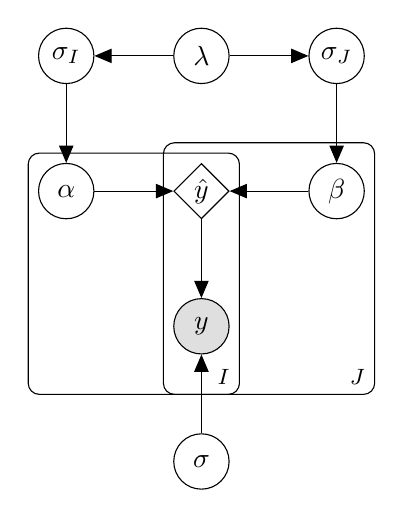
\begin{tikzpicture}

            \node[obs] (y) {$y$};
            \node[det, above=of y] (yhat) {$\hat{y}$};
            \node[latent, left=of yhat] (alpha) {$\alpha$};
            \node[latent, above=of yhat] (lambda) {$\lambda$};
            \node[latent, right=of yhat] (beta) {$\beta$};
            \node[latent, left=of lambda] (sigi) {$\sigma_I$};
            \node[latent, right=of lambda] (sigj) {$\sigma_J$};
            \node[latent, below=of y] (sigma) {$\sigma$};
            
            \edge {sigi} {alpha};
            \edge {sigj} {beta};
            \edge {sigma, yhat} {y};
            \edge {lambda} {sigi};
            \edge {lambda} {sigj};
            \edge {alpha,beta} {yhat};
        
            \plate {I} {(y)(yhat)(alpha)} {$I$};
            \plate {J} {(y)(yhat)(beta)(I.north east)} {$J$};
          
        \end{tikzpicture}}
        \caption{}
    \end{subfigure}
    \hspace{0.1in}
    \begin{subfigure}[b]{0.3\textwidth}

    \begin{minted}{julia}
m = @model I,J begin
    λ ~ HalfCauchy()
    σI ~ HalfNormal(λ)
    σJ ~ HalfNormal(λ)
     
    α ~ Normal(0, σI) |> iid(I)
    β ~ Normal(0, σJ) |> iid(J)
    yhat = α .+ β'

    σ ~ HalfNormal()
    y ~ For(I,J) do i,j 
            Normal(yhat[i,j], σ)
        end
    end
    \end{minted} 
    \caption{}
    \end{subfigure}

    \caption{A generative model (a), plate diagram (b), and Soss model (c) for a two-way analysis of variance model. Note the specification that $y$ will later be observed is not part of the model, but is instead given at inference time.}
    \label{fig:model}
\end{figure}

\subsection{Joint Distributions}

A Soss model is \emph{function-like}, taking values for its arguments and returning a \emph{joint distribution}. For example, given \jl#m# from Figure~\ref{fig:model}, we can build the joint distribution \jl#d=m(I=2, J=3)#. This supports the usual \jl#rand# and \jl#logpdf# functions, as well as some others provided by Soss described in the following sections. For example,\footnote{This and future examples are edited for space, for example rounding floating point values.}

\begin{minted}{julia}
julia> d = m(I=2, J=3); rand(d) # or rand(m(I=2, J=3))
(I = 2, J = 3, yhat = [-0.52 -1.5 0.0037; -0.81 -1.85 -0.28], σ = 2.5, λ = 1.3, σJ = 0.72, σI = 0.41, 
 β = [-0.54, -1.5, -0.023], α = [0.026, -0.26], y = [-0.45 -2.0 2.2; -3.4 -3.9 2.3])
\end{minted}

\subsection{Inference Primitives}

A given inference algorithm can be expressed in terms of a collection of functions on a model. For example, we may need to evaluate the log-density or its gradient, map continuous variables into $\mathbb{R}^n$, or draw random samples. In Soss, these \emph{inference primitives} generate model-specific code at execution time.

At this writing, the following inference primitive are available:

\todo[inline]{citation for MonteCarloMeasurements.jl}

\begin{description}  
    \item[\texttt{rand}] draws a random sample from a given joint distribution.
    \item[\texttt{particles}] draws a \emph{systematic sample} from a given joint distribution, using \texttt{MonteCarloMeasurements.jl}.
    \item[\texttt{logpdf}] takes a joint distribution and a point in its sample space, and returns the log-density.
    \item[\texttt{symlogpdf}] 
    \item[\texttt{weightedSample}] 
    \item[\texttt{xform}] 
\end{description}

\subsection{Model Transformations}


\subsubsection*{Conditional predictive models}




\subsubsection*{Causal interventions (``Do'' operator)}

\subsubsection*{Markov blankets}


\begin{minted}{julia}
julia> markovBlanket(m, :α)
    @model (I, σI, β, σ, J) begin
            α ~ Normal(0, σI) |> iid(I)
            yhat = α .+ β'
            y ~ For(I, J) do i, j
                    Normal(yhat[i, j], σ)
                end
        end 
\end{minted}


\subsection{Symbolic Manipulation}

\subsubsection*{Symbolic Log-density}

\subsubsection*{Code Generation}

\section{Implementation}

\begin{minted}{julia}
struct Model{A,B,M} 
    args  :: Vector{Symbol}
    vals  :: NamedTuple
    dists :: NamedTuple
    retn  :: Union{Nothing, Symbol, Expr}
end
\end{minted}


\section{Performance}

\todo[inline]{Let's implement models from \url{https://statisticalrethinkingjulia.github.io/MCMCBenchmarks.jl/latest/benchmarks/} for benchmark comparisons}

\todo[inline]{Can Soss really generate arbitrary code?}

The ability to generate arbitrary  Julia code makes it difficult to measure performance in Soss. When a performance bottleneck is found, developers or users can ask Soss to generate something different. This design places no a priori constraints on performance.

\todo[inline]{Restructure my writing?}

Besides the purely static code generation via regular macros happening in parsing time, Soss heavily uses a mechanism of "zero-cost" runtime code generation originated by Julia's generated functions \cite{bezanson2012julia}, a.k.a staged functions in the original paper and earlier versions of Julia Programming Language.

The generated functions provide the capability of performing code generation during type inference, generating programs computed by the body of function(a.k.a, generator), once and only once for each combination of argument types.

Further, Julia enables type inference and compiler optimizations equivalent to non-runtime ones in runtime for the callsites of generated functions, hence we gain runtime code generation without losing performance.

To take advantage of this, Soss designs a system to encode sufficient information for generating actual codes, into the types, or objects that can be dispatched like types, which allows the use of generated functions here.

Unfortunately, in current stage, there're some implementation restrictions to Julia's generated functions, and generated functions cannot generate arbitrary Julia codes,
where some advanced programming constructions are missing, such as generators and function-related stuffs like closures(including functions with no free variables), multiple dispatch, etc.

To address this, we introduced the works of easing the restrictions of Julia generated functions,
\todo[inline]{cite GG here?}
which allow us to generate closures from generated functions, and make the programs sufficiently powerful.

Programs that can be generated by Soss are turing complete, as all constructs of Lambda Calculus can be generated.

\begin{minted}{julia}
  abstract type LCTerm end
  struct Lam{Arg, Body <: LCTerm} <: LCTerm end
  struct App{Fn<:LCTerm, Arg<:LCTerm} <: LCTerm end
  struct Var{N} <: LCTerm end
  
  cg(::Type{Lam{Arg, Term}}) where {Arg, Term} = 
    :($Arg -> $(cg(Term)))
  cg(::Type{App{Fn, Arg}}) where {Fn, Arg} = 
    :($(cg(Fn))($(cg(Arg))))
  cg(::Type{Var{N}}) where N = N

  function tolc(expr)
    @match expr begin
      :($f($arg)) => App{tolc(f), tolc(arg)}
      :($x => $y) => Lam{x, tolc(y)}
      a::Symbol => Var{a}
    end
  end
  
  @gg function lc(::Type{Term}) where Term <: LCTerm
      cg(Term)
  end
  
  macro lc(term)
    lc(tolc(term))
  end
  
  x = Core.Box()
  y = Core.Box()
  z = Core.Box()
  f(x) = (x, z)
  @assert (@lc x => x)(x) === (@lc y => y)(x)
  @assert (@lc f => x => f(x))(f)(y) === (y, z)
  \end{minted} 



\section{Extending Soss}

\section{Related Work}

The idea of code generation and symbolic simplification in an embedded PPL goes back to \emph{Passage} \cite{Scherrer2012}. 

\emph{Hakaru} \cite{narayanan2016probabilistic} takes a more ambitious symbolic approach in a stand-alone PPL, allowing a wider variety of program transformations. 

Soss began with a goal of representing models with continuous, fixed-dimensionality parameter spaces, inspired by \emph{Stan} \cite{stan:2017}.

\emph{Gen} \cite{Cusumano-Towner:2019} was developed independently from Soss, but takes a similar approach (and distinct from most PPLs) in its representation of a model as a function from its arguments to a "trace" (to use Gen's terminology). In both Soss and Gen's static DSL, this trace is a mapping from variable names to values. The similarity of these systems makes interoperability relatively straightforward, as demonstrated in \emph{SossGen} (\url{https://github.com/cscherrer/SossGen.jl}).

\emph{Turing} \cite{ge2018t}

\begin{acks}
We would like to acknowledge...
\end{acks}

\bibliographystyle{acm-reference-format}
\bibliography{ref}

\appendix

\section{Model Syntax}

\begin{figure}[!t]
  \centering
  %\fbox{\rule[-.5cm]{0cm}{\linedwid} \rule[-.5cm]{4cm}{0cm}}
  % using the backnaur package
\begin{bnf*}
  \bnfprod{model}{\bnfts{@model} \bnfsp \bnfpn{args} \bnfsp \bnfts{begin} \bnfsp \bnfpn{statements} \bnfsp \bnfts{end}}\\
  \bnfprod{args}{\bnfes \bnfor \bnfpn{Symbol} \bnfor \bnfpn{Symbol} \bnfts{,} \bnfpn{args}} \\
  \bnfprod{statements}{\bnfpn{statement} \bnfor \bnfpn{statement} \bnfsp \bnftd{Julia Line Sep} \bnfsp \bnfpn{statements} \bnfor \bnfpn{statements} \bnfsp \bnfpn{retn}} \\ 
  \bnfprod{statement}{\bnfpn{assign} \bnfor \bnfpn{sample}} \\
  \bnfprod{assign}{\bnfpn{Symbol} \bnfsp \bnfts{=} \bnfsp \bnfpn{Expr}} \\
  \bnfprod{sample}{\bnfpn{Symbol} \bnfsp \bnfts{\textasciitilde}} \bnfsp \bnfpn{Measure} \\
  \bnfprod{retn}{\bnfts{return} \bnfsp \bnfpn{Expr}} \\
  \bnfprod{Symbol}{\bnftd{Julia Symbol}} \\ 
  \bnfprod{Expr}{\bnftd{Julia Expr}} \\
  \bnfprod{Measure}{\bnftd{Probability measure (see text)}}
\end{bnf*}
  \caption{Backus-Naur Form representation for a user-specified model.}
  \label{fig:bnf}
  \Description{Placeholder figure.}
\end{figure}

\section{Symbolic Simplification}

\begin{figure}[t!]
    \centering
    
    \begin{subfigure}[t]{0.4\textwidth}
        \[
    \begin{aligned}
        \ell = 
           &- 3 \log{\left(2 \right)} 
            - 5 \log{\left(\pi \right)} 
            - σ^{2} 
        \\ &- 4 \log{\left(λ \right)} 
            - 2 \log{\left(λ^{2} + 1 \right)} 
            - \frac{σ_I^{2}}{λ^{2}} 
            - \frac{σ_J^{2}}{λ^{2}}
        \\ &+ \sum_{i=1}^{I} \left(- \log{\left(σ_I \right)} - \frac{\log{\pi }}{2} - \frac{\log{2 }}{2}     - \frac{{α}_{i}^{2}}{2 σ_I^{2}}\right) 
        \\ &+ \sum_{j=1}^{J} \left(- \log{\left(σ_J \right)} - \frac{\log{\pi }}{2} - \frac{\log{2 }}{2}     - \frac{{β}_{j}^{2}}{2 σ_J^{2}}\right) 
        \\ &+ \sum_{\substack{1 \leq i \leq I \\ 1 \leq j \leq J}} \left(- \log{\left(σ \right)} - \frac    {\log{\pi }}{2} - \frac{\log{2 }}{2} - \frac{\left({y}_{ij} - {\hat{y}}_{ij}\right)^{2}}{2 σ^{2}    }\right) 
    \end{aligned}
    \]
    \caption{Before}
    \end{subfigure}
    \hfill
    \begin{subfigure}[t]{0.4\textwidth}
        \[
    \begin{aligned}
    \ell =
    &- 7.8 - 0.92 I - 0.92 J - 0.92 I J - σ^{2} 
    \\ &- 4 \log{λ } - 2 \log{\left(λ^{2} + 1 \right)} 
        - I J \log{σ } 
    \\ &- I \log{σ_I } - J \log{σ_J } - \frac{σ_I^{2}}{λ^{2}}  - \frac{σ_J^{2}}{λ^{2}}
    \\ &- \frac{1}{2 σ_I^{2}} \sum_{i=1}^{I} {α}_{i}^{2}
        - \frac{1}{2 σ_J^{2}} \sum_{j=1}^{J} {β}_{j}^{2}
    \\ &- \frac{1}{2 σ^{2}} \sum_{\substack{1 \leq i \leq I\\1 \leq j \leq J}} \left({y}_{ij} - {\hat{y}}_{ij}\right)^{2}
    \end{aligned}
\]
    \captionsetup{skip=27pt}
    \caption{After}
    \end{subfigure}
    \caption{Symbolic log-density of $m$ before (a) and after (b) simplification steps. Reduction }
    \label{}
\end{figure}

Before simplification:


After simplification:



\section{Extended example }
\todo[inline]{Break this up! This is just a staging area}

\begin{minted}{julia}
julia> using Revise, Soss, Random

julia> Random.seed!(1);

julia> m = @model I,J begin
           λ ~ HalfCauchy()
           σI ~ HalfNormal(λ)
           σJ ~ HalfNormal(λ)
           α ~ Normal(0, σI) |> iid(I)
           β ~ Normal(0, σJ) |> iid(J)
           yhat = α .+ β'
           σ ~ HalfNormal()
           y ~ For(I,J) do i,j 
                   Normal(yhat[i,j], σ)
               end
       end;

julia> truth = rand(m(I=2,J=3)); pairs(truth);

julia> post = dynamicHMC(m(I=2,J=3), (y=truth.y,));

julia> postpred = predict(m(I=2,J=3), post) |> particles;

julia> postpred.yhat
2×3 Array{Particles{Float64,1000},2}:
 0.241 ± 0.26  0.527 ± 0.3   -0.556 ± 0.38
 0.22 ± 0.26   0.506 ± 0.32  -0.577 ± 0.37

julia> postpred.y
2×3 Array{Particles{Float64,1000},2}:
 0.224 ± 0.58  0.529 ± 0.58  -0.58 ± 0.64
 0.223 ± 0.56  0.483 ± 0.58  -0.58 ± 0.61

julia> m.args
2-element Array{Symbol,1}:
 :I
 :J

julia> pairs(m.vals)
pairs(::NamedTuple) with 1 entry:
  :yhat => :(α .+ β')

julia> pairs(m.dists)
pairs(::NamedTuple) with 7 entries:
  :λ  => :(HalfCauchy())
  :σI => :(HalfNormal(λ))
  :σJ => :(HalfNormal(λ))
  :α  => :(Normal(0, σI) |> iid(I))
  :β  => :(Normal(0, σJ) |> iid(J))
  :σ  => :(HalfNormal())
  :y  => :(For(I, J) do i, j…

\end{minted}

\end{document}
